\section{Модел на Ross}
\begin{frame}[t]{Ronald Ross}
  Роден през 1857 в Индия син на английски офицер.

  Получава медицинско образование в Англия, а преди това се образова по многобройни теми, включително математика.

  След поредица експерименти през 90-те години на XIX век, Ronald Ross открива плазмодия в слюнчестите жлези на комари от род \textit{Anopheles}.

  За приноса си става носител на Нобеловата награда за физиология или медицина през 1902г.

  Лансира идеята за намаляване на популацията комари като начин за справяне с маларията.

  Почива през 1932 г.
\end{frame}

\begin{frame}[t]{Ronald Ross}
  \begin{figure}
    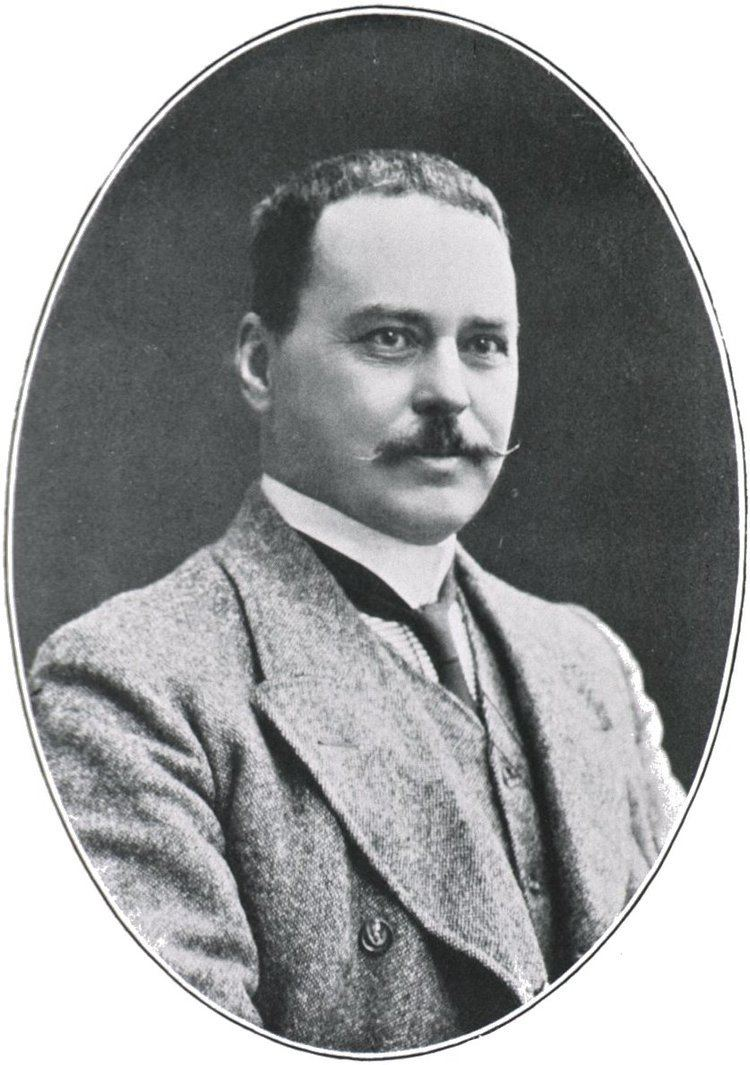
\includegraphics[width=0.7\textwidth, height=0.75\textheight]{ronald-ross-e053ee1d-92ea-4ae9-a175-9a4ce0d7ac4-resize-750.jpg}
    \centering
    \caption{Sir Ronald Ross, 1857-1932}
  \end{figure}
\end{frame}

\begin{frame}[t]{Модел на Ross}
  Допускания на модела:
  \begin{enumerate}
    \item Заразен човек/комар не може да бъде заразен повторно.
    \item Хората могат да оздравеят от заразата, а комарите - не.
    \item Комарите извършват константен брой ухапвания за единица време.
    \item Популационната динамика на хората се пренебрегва.
    \item Популациите на хората и комарите са константни.
  \end{enumerate}
\end{frame}

\begin{frame}[t]{Модел на Ross}
  Означения:
  \begin{enumerate}
    \item $X(t)$ е броя заразени с малария хора в момент $t$.
    \item $Y(t)$ е броя заразени с малария комари в момент $t$.
    \item $N$ е човешката популация.
    \item $M$ е популацията от комари.
    \item $\gamma$ е скоростта на оздравяване на хората.
    \item $\mu$ е скоростта на смъртност на комарите.
    \item $b$ е честотата на ухапване на комарите за единица време.
    \item $\beta_{vh}$ е константна вероятност за заразяване на здрав човек с патогена, когато бъде ухапан от заразен комар, а $\beta_{hv}$ е константна вероятност за заразяване на здрав комар с патогена, когато ухапе заразен човек.
  \end{enumerate}
\end{frame}

\begin{frame}[t]{Модел на Ross}
  За интервал $\Delta t$:

  Заразените хора ще се получат, като се вземат всички ухапвания на заразени комари за периода $b Y(t) \Delta t$ и се умножат по вероятността да са по незаразен човек $\frac{N-X(t)}{N}$, както и да се предаде патогена $\beta_{vh}$, т.е. $b  Y(t) \Delta t \frac{N-X(t)}{N} \beta_{vh} $, а оздравелите ще са $\gamma X(t) \Delta t$.

  За този интервал пък заразените комари ще се получат, като се вземат всички ухапвания от незаразени комари $b (M - Y(t)) \Delta t$ и се умножат по вероятнстта да са по заразен човек $\frac{X(t)}{N}$, както и да се предаде патогена $\beta_{hv}$, т.е. $b (M - Y(t)) \Delta t \frac{X(t)}{N} \beta_{hv} $, а умрелите ще са $\mu Y(t) \Delta t$.

  След деление на $\Delta t$ и граничен преход се достига до следния модел:
\end{frame}

\begin{frame}[t]{Модел на Ross}
  \begin{equation}
    \label{eq:BasicProblem}
    \begin{split}
      &\dot{X}(t) = \beta_{vh} b \frac{N-X(t)}{N} Y(t) - \gamma X(t) \\
      &\dot{Y}(t) = \beta_{hv} b \frac{X(t)}{N} (M-Y(t)) - \mu Y(t) \\
    \end{split}
  \end{equation}
  Вижда се, че $(0, 0)$ е равновесна точка за \eqref{eq:BasicProblem}.

  Може да има ендемична равновесна $E^* = (X^*, Y^*)$:
  \begin{equation*}
    E^* = (X^*, Y^*) = \left(N \frac{1 - \frac{\gamma \mu N}{b^2 \beta_{vh} \beta_{hv} M}}{1 + \frac{\gamma N}{b \beta_{vh} M}}, M \frac{1 - \frac{\gamma \mu N}{b^2 \beta_{vh} \beta_{hv} M}}{1 + \frac{\mu}{b \beta_{hv}}}\right)
  \end{equation*}
  За да съществува, координатите ѝ трябва да са положителни.
\end{frame}

\begin{frame}[t]{Модел на Ross}
  Заключения на Ross:
  \begin{enumerate}
    \item За да съществува $E^*$ е необходимо $M > M^* = \frac{\gamma \mu N}{b^2 \beta_{vh} \beta_{hv}}$.
    \item Ако се намали броя на комари под $M^*$, маларията ще изчезне след време.
      % \item При $\frac{M}{N}$ малко над $\frac{M^*}{N}$, $\frac{X^*}{M}$ достига стойност, от която малко се мени за по-големи $\frac{M}{N}$. Това обяснява практически наблюдения, че пропорцията заразени почти не зависи от многобройността на комарите.
    \item При $\frac{M}{N}$ малко над $\frac{M^*}{N}$, $\frac{X^*}{N}$ бързо расте, а после много по-бавно за по-големи $\frac{M}{N}$. Така връзката между брой комари и наличието на малария не е била лесна за намиране чисто практически.
      % Това обяснява дотогавашните практически наблюдения, че пропорцията заразени почти не зависи от многобройността на комарите.
  \end{enumerate}

  С това изследване Ross доказва разсъжденията си за изкореняването на маларията.
\end{frame}
